\documentclass[letterpaper, 10 pt, conference]{ieeeconf}  % Comment this line out if you need a4paper
%\documentclass[a4paper, 10pt, conference]{ieeeconf}      % Use this line for a4 paper
\IEEEoverridecommandlockouts                              % This command is only needed if 
                                                          % you want to use the \thanks command
\overrideIEEEmargins                                      % Needed to meet printer requirements.

\usepackage[pdftex]{graphicx}
\usepackage{algpseudocode}
\usepackage[noadjust]{cite}

\title{\LARGE \bf
  Longitudinal Trajectory Planning and Tracking for Fixed-Path Autonomous Driving
}

\author{
  Robert G. Cofield $^{1}$,
  Rakesh Gupta $^{2}$,
  Ambarish Goswami $^{3}$,
  and
  David Bevly $^{4}$
  \thanks{
    * This work is supported by Honda Research Institute USA.
  }
  \thanks{
    $^{1}$ Robert G. Cofield is a graduate researcher at Auburn University's GPS \& Vehicle Dynamics Laboratory.
  }
  \thanks{
    $^{2}$ Rakesh Gupta ...
  }
  \thanks{
    $^{3}$ Ambarish Goswami ... 
  }
  \thanks{
    $^{4}$ David Bevly ...
  }
}


%%%%%%%%%%%%%%%%%%%%%%%%%%%%%%%%%%%%%%%%%%%%%%%%%%%%%%%%%%%%%%%%%%%%%%%%%%%%%%%%
%%%%%%%%%%%%%%%%%%%%%%%%%%%%%%%%%%%%%%%%%%%%%%%%%%%%%%%%%%%%%%%%%%%%%%%%%%%%%%%%
%%%%%%%%%%%%%%%%%%%%%%%%%%%%%%%%%%%%%%%%%%%%%%%%%%%%%%%%%%%%%%%%%%%%%%%%%%%%%%%%

\begin{document}

\maketitle
\thispagestyle{empty}
\pagestyle{empty}

%%%%%%%%%%%%%%%%%%%%%%%%%%%%%%%%%%%%%%%%%%%%%%%%%%%%%%%%%%%%%%%%%%%%%%%%%%%%%%%%
\begin{abstract}

When planning trajectories for an autonomous ground vehicle operating on roadways, it is common to employ the path-velocity decomposition (i.e., path planning is performed prior to planning the speed that the vehicle will take along the chosen path).
Given a desired path, we present a novel method of planning longitudinal trajectories (i.e., the time derivatives of position in the body-forward direction) along that path.
This method first segments the path using an arbitrary set of kinematic or dynamic constaints which may be functions of the desired path.
Each segement is then planned sequentially by choosing a piecewise constant jerk profile.
The jerk profile is intelligently chosen from a set of pre-solved profiles such that acceleration is continuous throughout the entire path.
The resultant trajectory plan can then be easily sampled to provide a reference for real-time vehicle control.
This method is shown to be efficient and reliable for use in online planning with a test vehicle.

\end{abstract}
%%%%%%%%%%%%%%%%%%%%%%%%%%%%%%%%%%%%%%%%%%%%%%%%%%%%%%%%%%%%%%%%%%%%%%%%%%%%%%%%

%%%%%%%%%%%%%%%%%%%%%%%%%%%%%%%%%%%%%%%%%%%%%%%%%%%%%%%%%%%%%%%%%%%%%%%%%%%%%%%%
\section{Introduction} \label{sec:introduction}

... autonomous vehicles ... \emph{The 1st sentence is the hardest}.
One such task is computing a tentative reference trajectory plan for travelling from one point to another.
While the set of possible paths between any two points is infinite, it is typically heavily restricted by consideration of constraints such as traversability and legally available travel lanes, among others.
The intended speed, acceleration, and higher derivates of position with respect to time are also subject to constraints.
These may include legal speed limits, engine dynamics, desired sideslip limits, traction availability, and rollover concerns.

% intersection of path-planning constraints and speed-planning constraints is vehicle dynamics

% review of literature for a few paragraphs]
%  - searching planners (OMPL stuff)
%  - robot joint planning --> constant jerk intervals

% We will use the path-velocity decomposition
% mention using curvilinear CS
% 

Lit review...

% tracking
Once a trajectory plan is formulated, it must be utilized online in order for a reference signal to be sent to the controllers which govern steering, braking, and engine speed.
This is the trajectory tracking problem, which is discussed in Section \ref{sec:trajectorytracking}.

How is this different from the others ...

% mention using same cuvilinear cs scheme to project onto path

\section{Trajectory Planning} \label{sec:trajectoryplanning}

For the purposes of this work, the objective of trajectory planning is to take a 2 dimensional (horizontal plane) path, and compute a series of constant jerk intervals for motion along the length of the path which is time optimal yet still falls within constraints on speed, acceleration, and jerk.
Integrating piecewise constant jerk over time yields acceleration which is piecewise linear over time, speed which is piecewise quadratic over time, and position which is piecewise cubic over time.
It is assumed that the path planner operates independently from the trajectory planner and tracker.
Prescribed initial and end conditions for position, speed, and acceleration must also be honored. 
This means that the desired trajectory plan is one dimensional, so using curvilinear coordinates will significantly simplify the solution.

\begin{figure}[thpb]
  \centering
  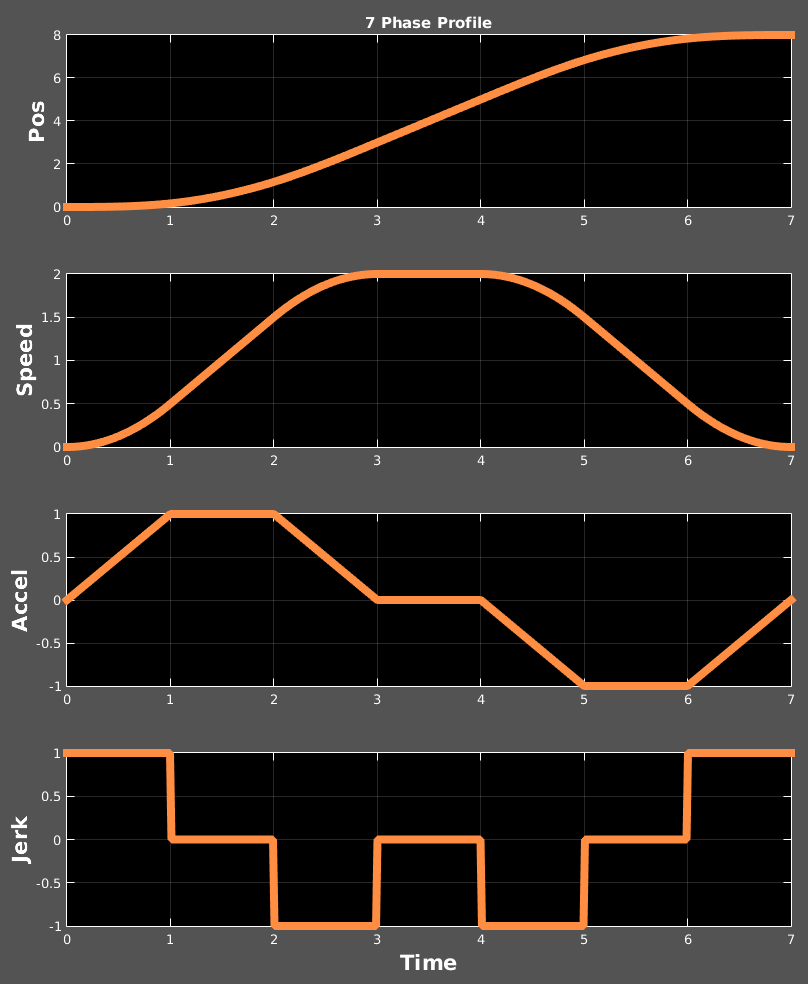
\includegraphics[width=1.0\columnwidth]{graphics/7phaseprofile.png}
  \caption{7 phase constant jerk profile along curvilinear distance axis.}
  \label{fig:7phaseprofile}
\end{figure}

\subsection{Jerk Profiles} \label{sec:jerkprofiles}

Consider, as a starting point, the case in which a vehicle is at rest and needs to accelerate to some travelling speed, maintain that speed for some distance, then brake to a stop at a prescribed end location.
Figure \ref{fig:7phaseprofile} shows this trajectory over time.
The problem is defined by the vector of known values $\mathbf{b}  = [v_i, a_i, L, v_m, v_f]$, being initial speed, initial acceleration, the total distance, speed limit, and the final speed, respectively.
If the magnitude of the desired peak acceleration and jerk ($a_m$ and $j_m$, respectively) are known, then the profile with $M$ jerk phases (7 in this case) can be generated by solving for the time intervals $[\Delta t_1, ..., \Delta t_M]$.
Jerk and peak acceleration may be different when reducing speed versus increasing speed to more closely mirror human driving behavior \emph{Citation}.
The remaining parameters yet to be set now become $\mathbf{a}_m = [a^+_m , a^-_m]$ and $\mathbf{j}_m = [j^+_m , j^-_m]$.
There are, however, multiple solutions for $\Delta t_2$, $\Delta t_4$, and $\Delta t_6$.
The proper solution must be chosen by eliminating negative and complex solutions.

It is obvious that there are many cases in which this solution will fail.
For instance, if $L$ is sufficiently short and $v_m$ is sufficiently high, then it will not be possible to ever reach $v_m$ with realistic values of $\mathbf{a}_m$ and $\mathbf{j}_m$.
The authors then propose that 4 other basic profiles be defined, and an algorithm constructed which judiciously chooses the appropriate profile for every segment defined by a vector $\mathbf{b}$.
The other profiles are explained below in section \ref{sec:jerkprofiles}.
A path is then a set of $N_s$ segments, each of which is defined by a set of parameters $\mathbf{b}_k, k = 1 ... N_s$ and can be solved indivually in sequence.
Determination of where to break a path into segments is discussed below in Section \ref{sec:pathsegmentation}.

There are a total of five potential jerk profiles which have been created to cover all feasible values in $\mathbf{b}$. All impossible scenarios are automatically ruled out.

\subsubsection{6 Phase} \label{sec:6phase}

In the case mentioned above, the speed limit is too high for a solution to exist for a 7 phase profile.
The middle travel period is removed, so that the vehicle increases speed and then immediately decreases speed. 
The peak speed in this case has a solution, but cannot be manipulated directly.

\begin{figure}[thpb]
  \centering
  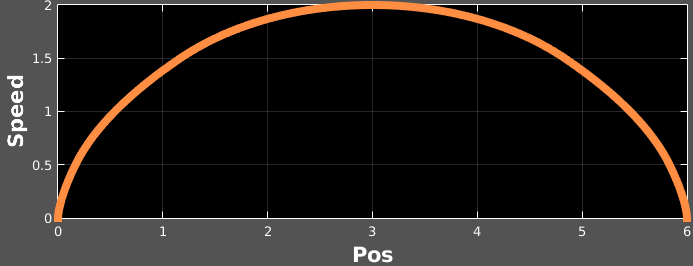
\includegraphics[width=0.7\columnwidth]{graphics/6phase_v(s).png}
  \caption{6 phase profile, displayed as speed vs. position along path}
  \label{fig:6phaseprofile}
\end{figure}

\subsubsection{4 Phase} \label{sec:4phase}

When $v_i < v_m \simeq v_f$, the vehicle should increase speed, then maintain that speed for the distance remaining in the segment.

\begin{figure}[thpb]
  \centering
  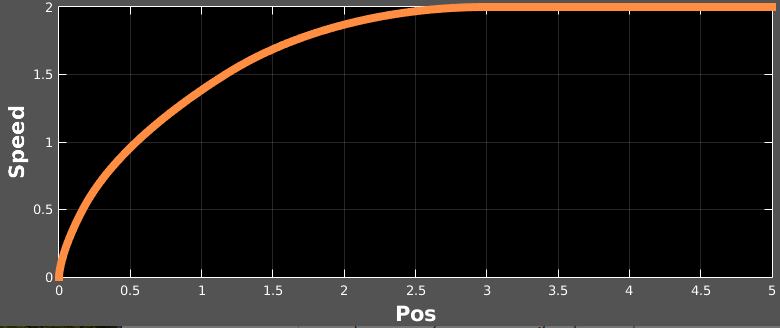
\includegraphics[width=0.7\columnwidth]{graphics/4phase_v(s).png}
  \caption{4 phase profile, displayed as speed vs. position along path.}
  \label{fig:4phaseprofile}
\end{figure}

\subsubsection{Reversed 4 Phase} \label{sec:reversed4phase}

When $v_i \simeq v_m > v_f$, it would be nonsensical to immediately brake.
The initial speed is maintained for a period before applying the brakes.

\begin{figure}[thpb]
  \centering
  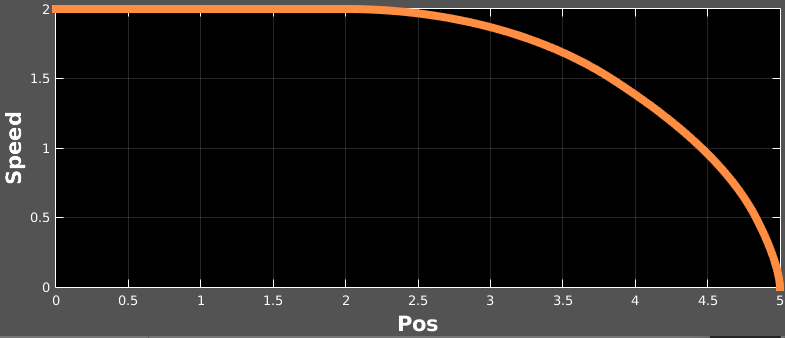
\includegraphics[width=0.7\columnwidth]{graphics/4Rphase_all_derivatives.png}
  \caption{Reversed 4 phase profile, displayed as speed vs. position along path.}
  \label{fig:4rphaseprofile}
\end{figure}

\subsubsection{3 Phase} \label{sec:3phase}

A change from one speed to another. 
This presents a difficulty in that either $L$ or $v_f$ may be enforced, but not both (there is no solution to enforce both).
As such, this profile is chosen for a segment in which it is impossible to completely arrive at the end speed given the initial speed. 

\begin{figure}[thpb]
  \centering
  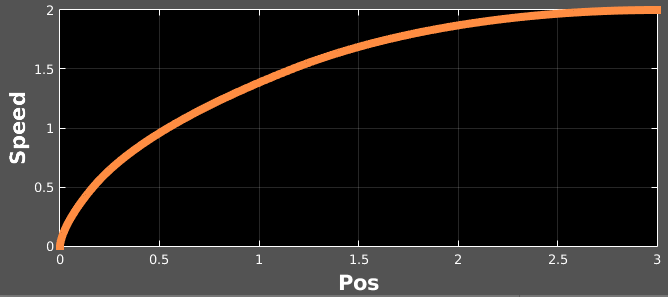
\includegraphics[width=0.7\columnwidth]{graphics/3phase_v(s).png}
  \caption{3 phase profile, displayed as speed vs. position along path.}
  \label{fig:3phaseprofile}
\end{figure}

To decide which profile to employ, a cascade approach is used.
Analytic values of time intervals are evaluated for each profile by plugging in values of $\mathbf{b}$, $\mathbf{a}_m$, and $\mathbf{j}_m$ until all time intervals are positive and real. 
The order in which they are attempted is: 7 $\rightarrow$ 6 $\rightarrow$ 4 $\rightarrow$ 4R $\rightarrow$ 3.

\emph{Put kinematic equations here? Many are extrememly large, and I don't have the code. Perhaps better to summarize what was put into the symbolic solver.}

\subsection{Path Segmentation} \label{sec:pathsegmentation}

% make sure to incorporate extensibility to other constraints
The goal of the segmentation process is to divide a given path into multiple portions where each has a uniform upper limit on speed, acceleration, and braking.
There are 3 steps in the segmentation process:
\begin{enumerate} \label{asdf}
  \item \emph{Ceiling calculation}, where $\mathbf{b}$, $\mathbf{a}_m$, and $\mathbf{j}_m$ are found for every point in the given path.
  \item \emph{Clustering}, in which path points are grouped sequentially.
  \item \emph{Consolidation}, in which a single $\mathbf{b}$, $\mathbf{a}_m$, and $\mathbf{j}_m$ is selected for each segment.
\end{enumerate}
After this is done, the process described above in Section \ref{sec:jerkprofiles} may be applied to each of the segments.

The ceiling calculation is a minimax problem.
Each of the 9 scalars is a minimum of several maxima computed from an arbitrary set of constraints.
For instance, ... \emph{put examples of things we didn't do...}

% How we actually did this.
For the purposes of developing a simple example application, two constraints will be used for $v_{m,k}$: legal speed limit ( $SL$, set constant for the whole path) and lateral acceleration limit ($a_{B,y}^{max}$. 
Lateral acceleration constraints are translated into longitudinal speed constraints using the approximation $v_{m,k}(a_{B,y}) = \sqrt{a_{B,y}^{max}/\kappa_k}$ for $k = 1, ..., N_p$.
For each path point, the value $v_{m,k}(a_{B,y}^{max})$ denotes the speed necessary to obtain the limit lateral acceleration, denoted by $a^{max}_{B,y}$.
The value $\kappa_k$ denotes the path curvature at each point.

This information is used to choose the segment boundaries in the clustering step.
Any number of clustering algorithms may be used here, and prudent choice of segment boundaries is arguably one of the most critical pieces of trajectory planning process.
For the present example, we will choose a simple univariate heuristic which essentially identifies curves in the roadway.
Each time that $v_{m,k} < SL$ becomes true, a curve is beginning, and a segment boundary is drawn.
Each time that $v_{m,k} = SL$ is once again true, the current curve has ended, and another segment boundary is drawn.
Figure \ref{fig:course_highlight_turns} shows the result of this algorithm. 

\begin{figure}[thpb]
  \centering
  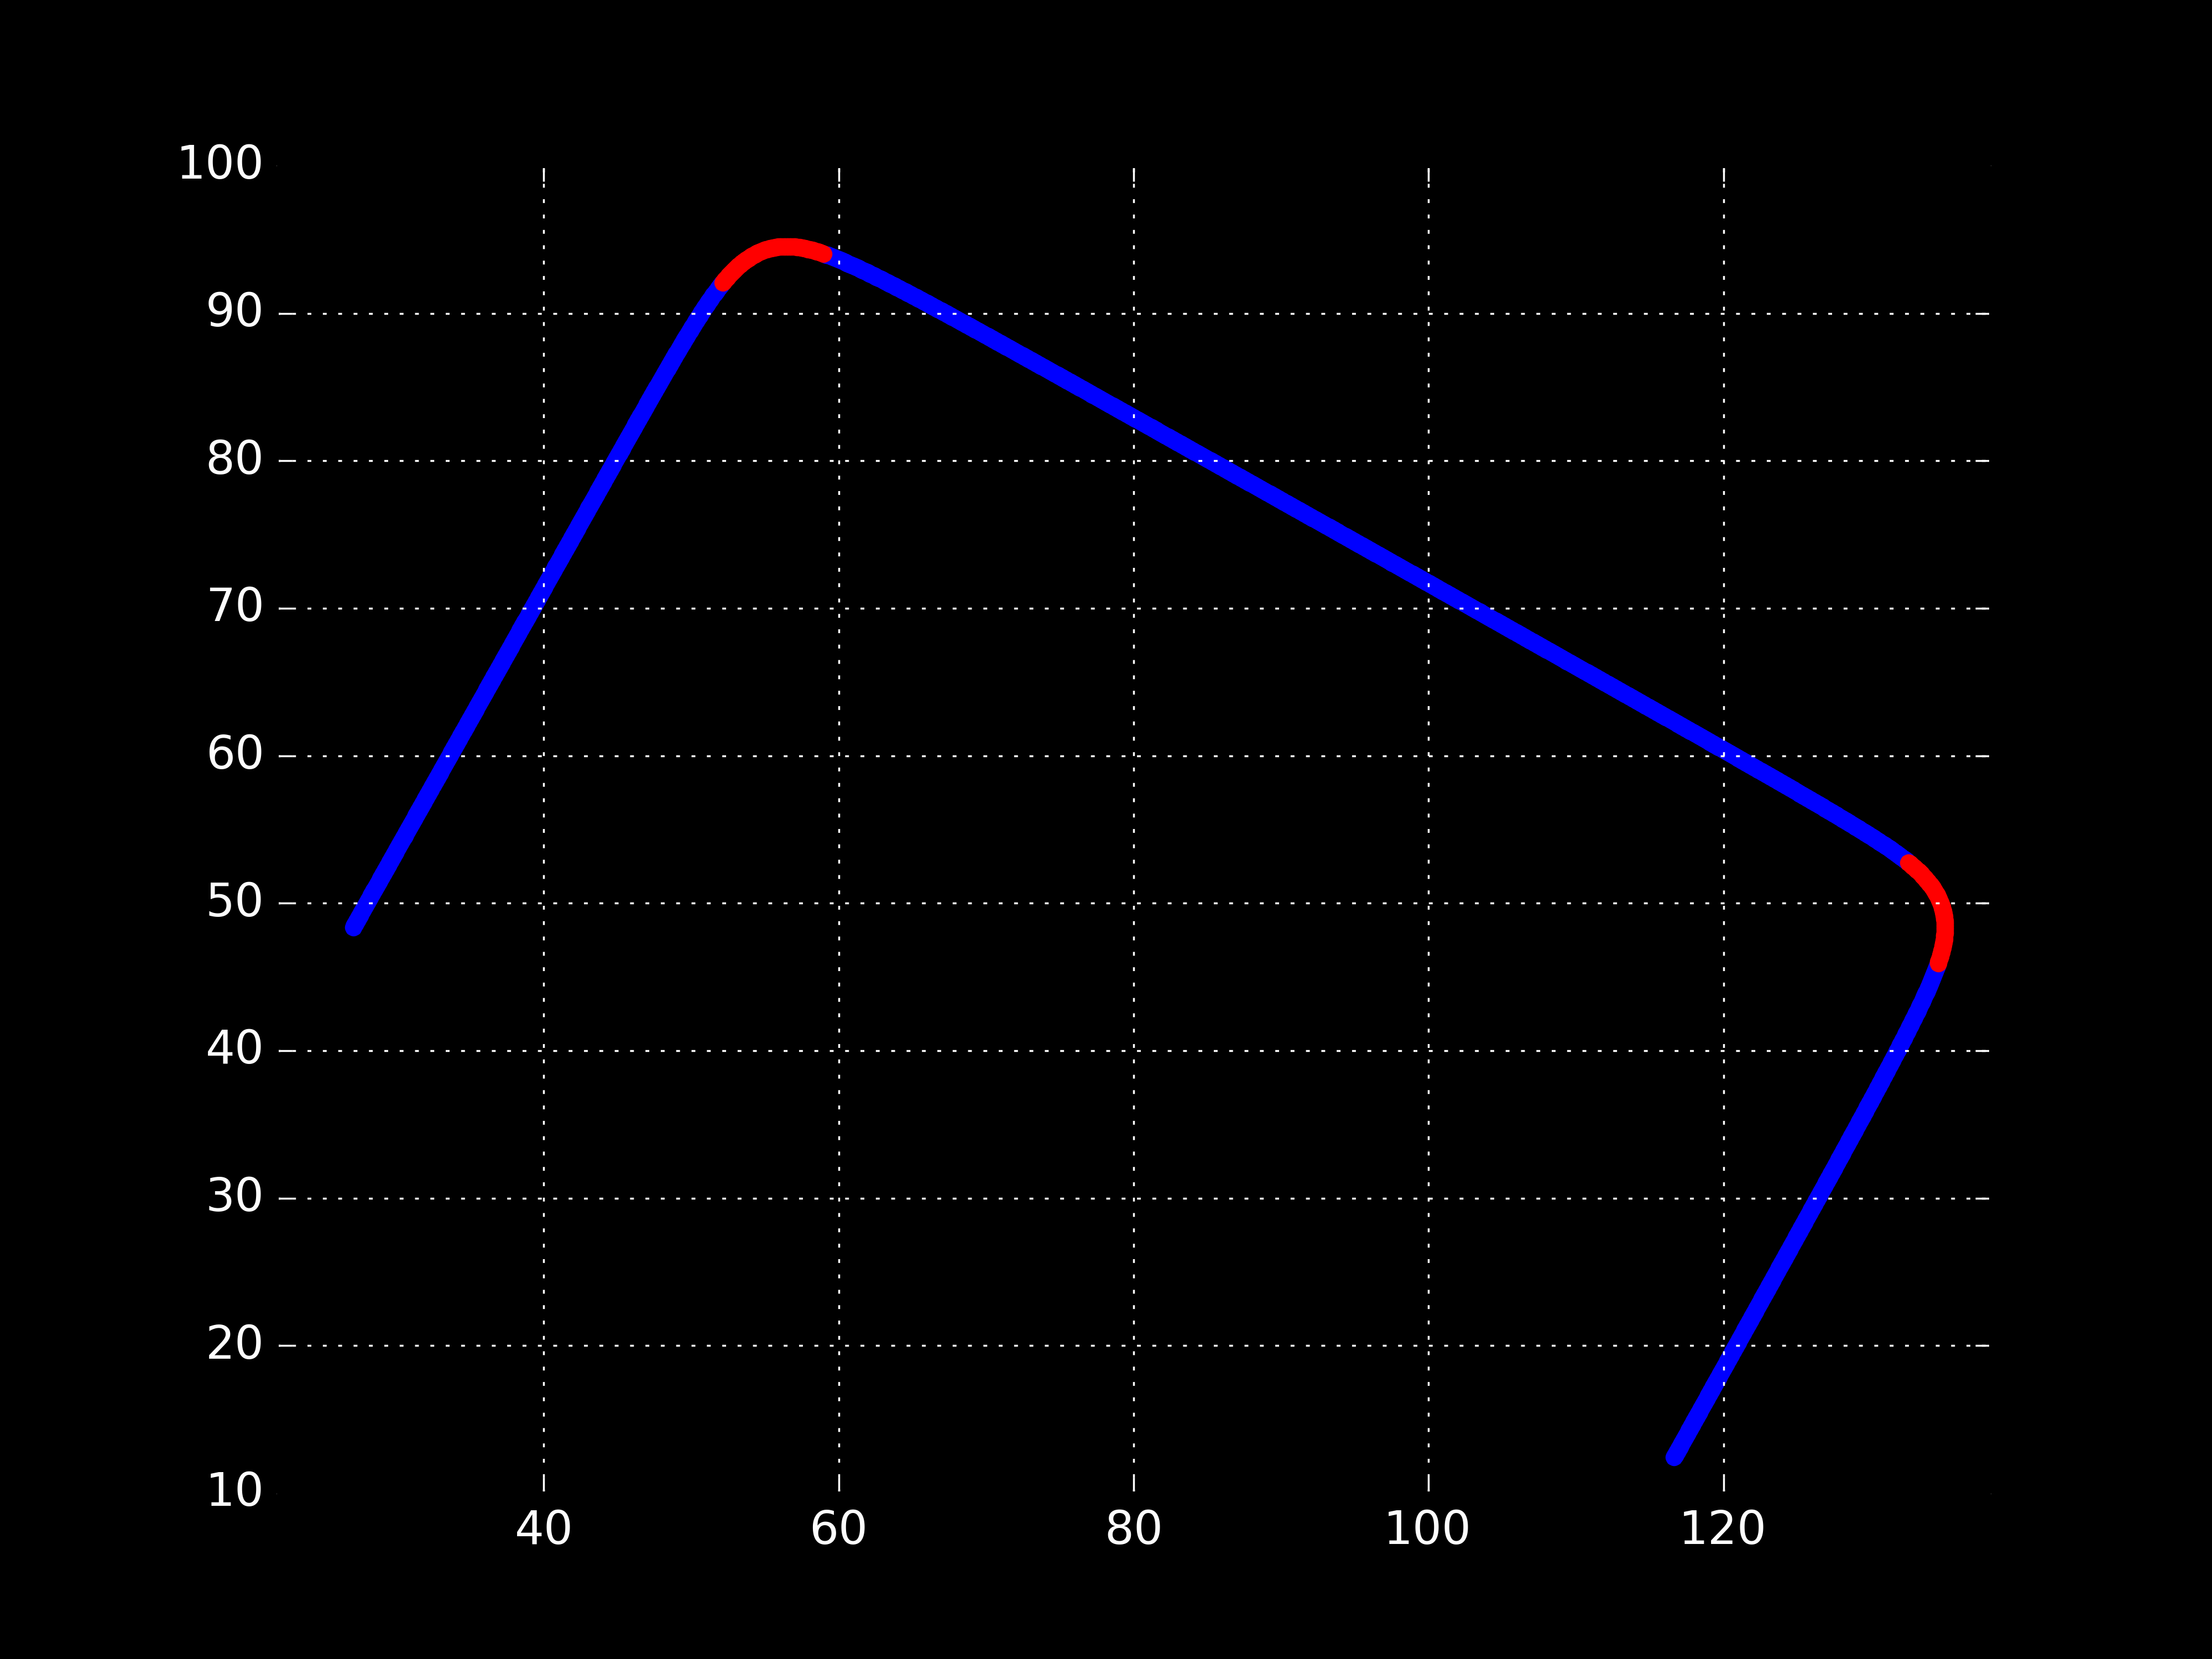
\includegraphics[width=0.8\columnwidth]{graphics/course_highlighted_turns.png}
  \caption{Clustering output for a short path when using an algorithm which draws segment boundaries around curves.}
  \label{fig:course_highlight_turns}
\end{figure}

% need better notation here.
In the consolidation step, a single set of $\mathbf{g}$, $\mathbf{a}_m$, and $\mathbf{j}_m$ must be calculated for each segment using the values corresponding to each of the path points which comprise the segment in question.
The minimum of scalar across all constituent points is chosen.
While not time optimal, it does ensure that no constraints are violated while still keeping the number of total segments low.
In the present example, this means that in the straight portions of the path $v_m = SL$ and in the curves $v_m$ is set to the value required to obtain $a_{B,y}^{max}$ for the entireity of the curve.
As a result, many of the curves will have a constant speed.
For the sake of simplicity, the values of $a^+_{m,k}$, $a^-_{m,k}$, $j^+_{m,k}$, and $j^-_{m,k}$ are all set constant for the entire path, using values from \cite{Maurya2012,Hoberock1977,Long2000}.

\begin{figure}[thpb]
  \centering
  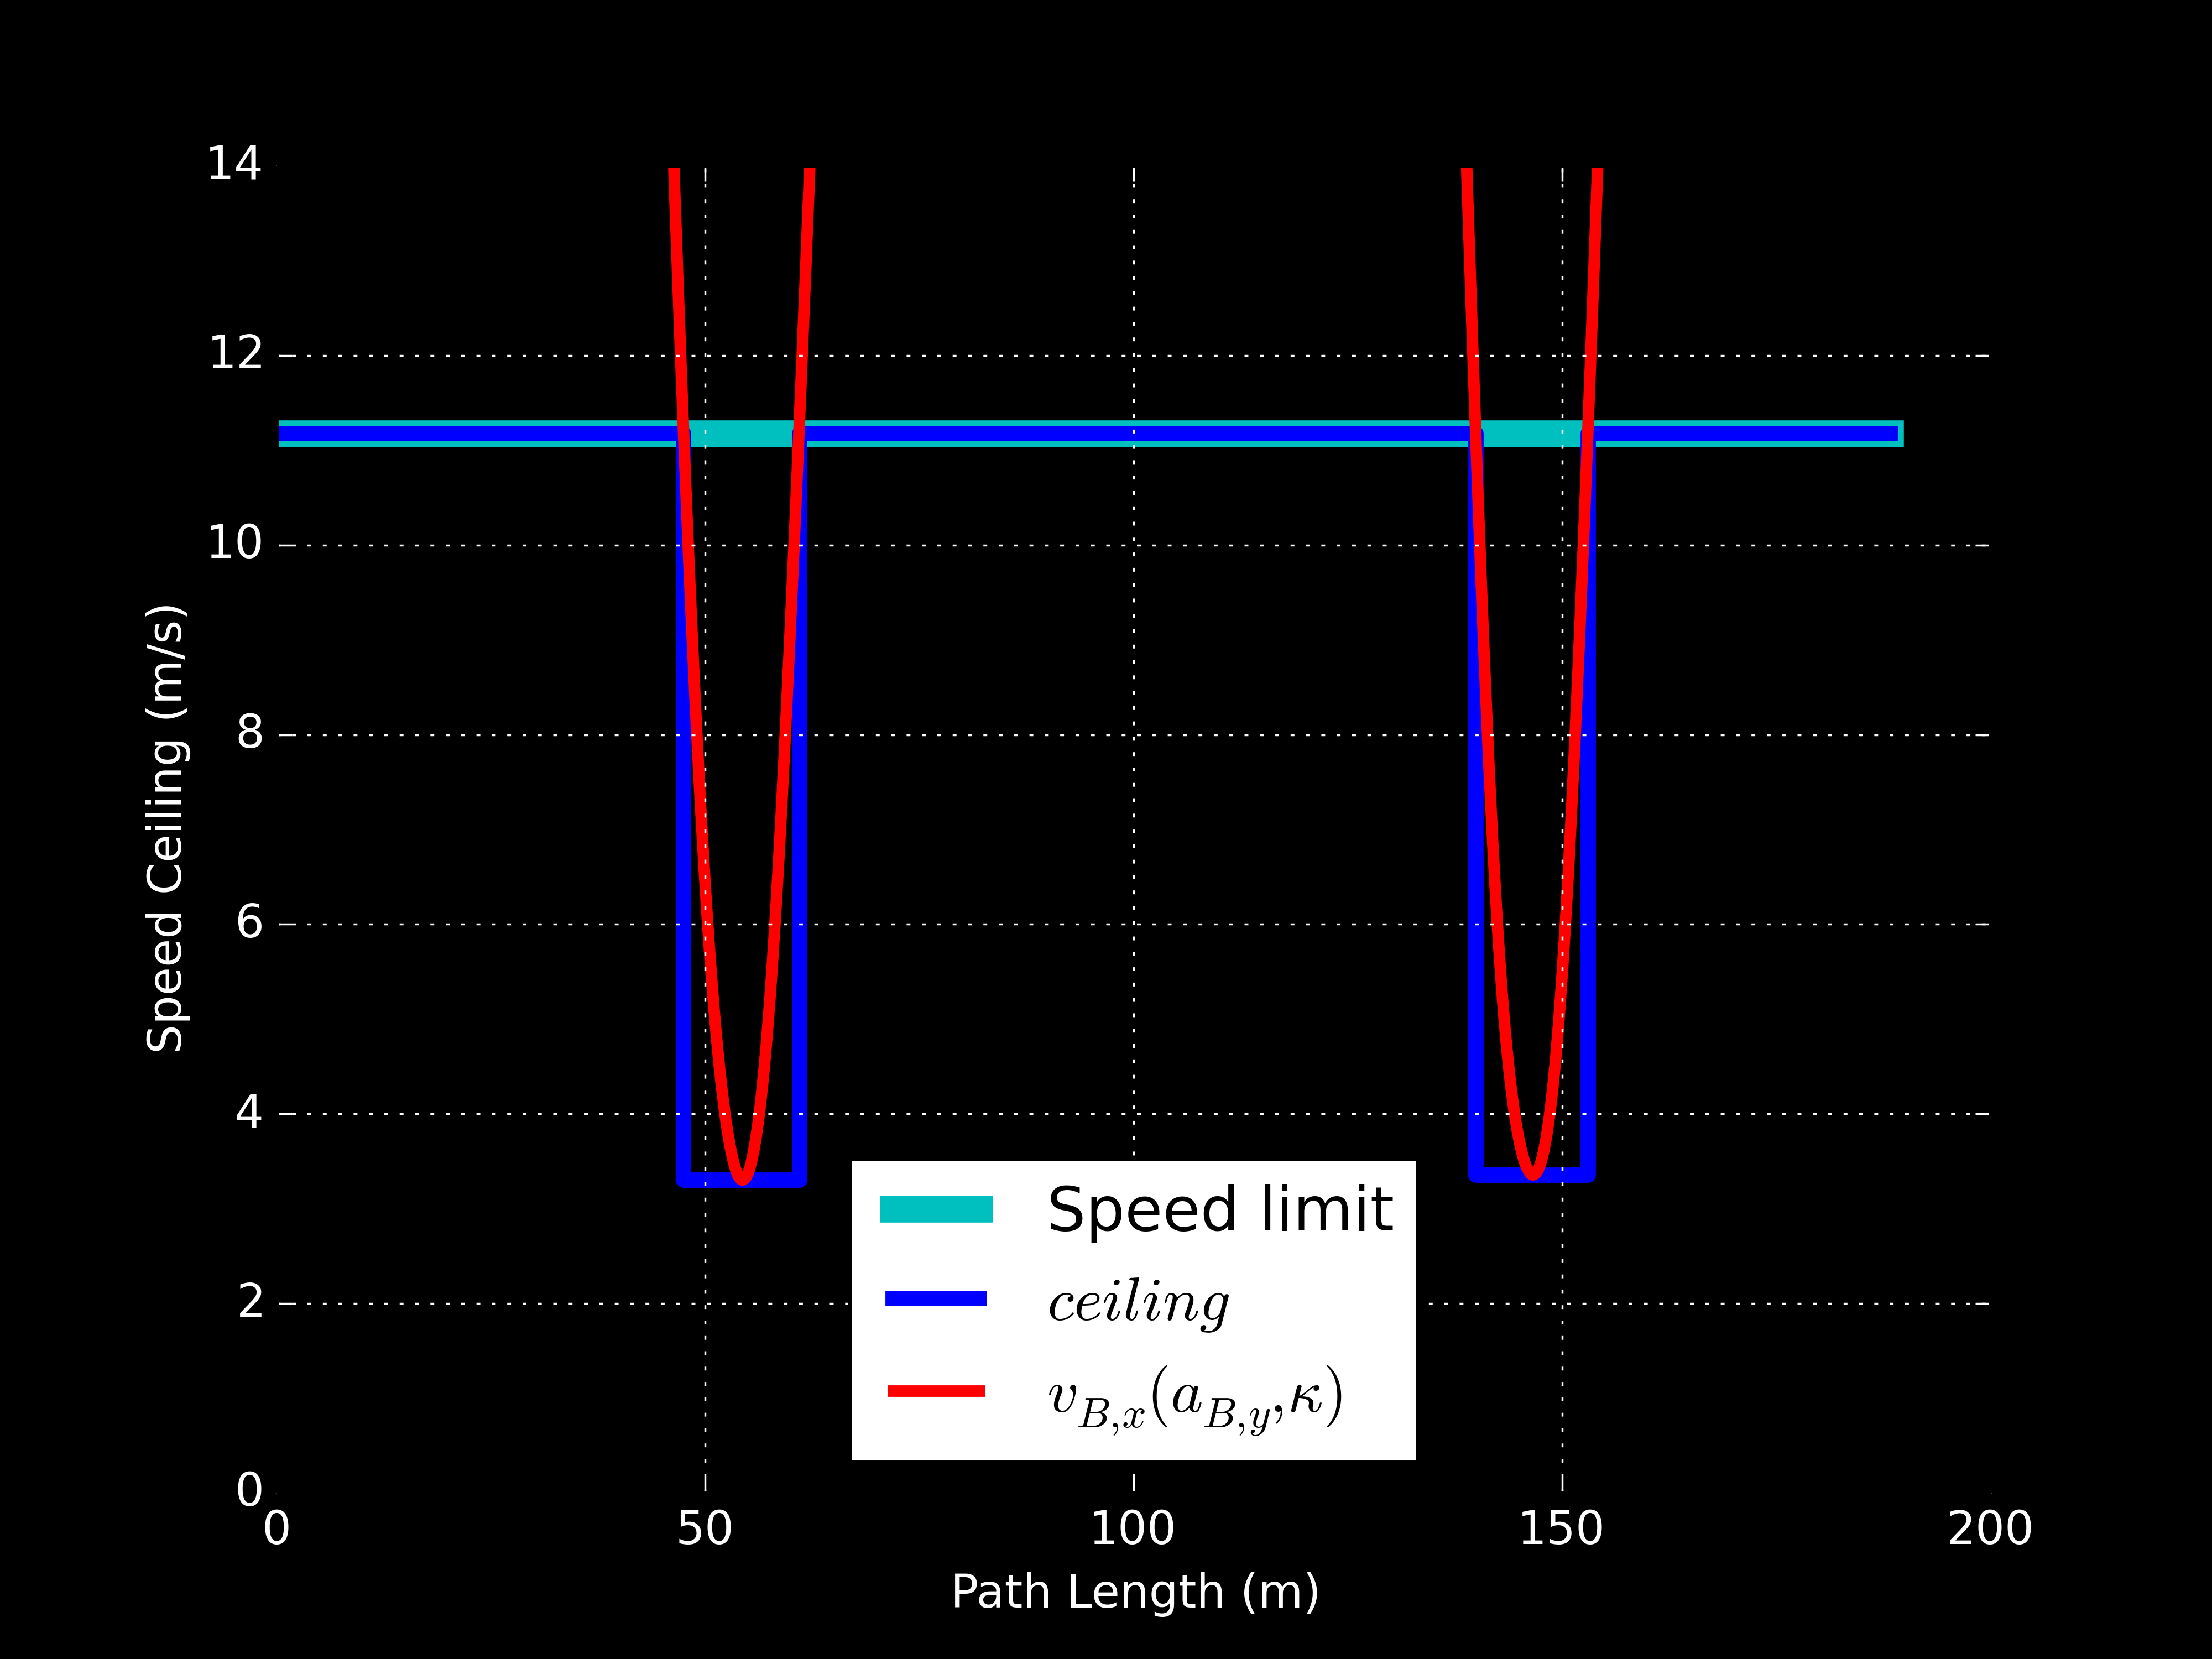
\includegraphics[width=0.8\columnwidth]{graphics/speed_ceiling.png}
  \caption{Example of $v_m$ consolidation for simple univariate path clustering.}
  \label{fig:consolidation_speed_ceiling}
\end{figure}

The power of this algorithm is that any set and number of constraints may be used ... \emph{etc., etc., ...}\tabularnewline

\subsection{Unified Solution} \label{sec:unifiedsolution}

At this point, the path has been divided into segments and conditions have been computed such that an analytically derived plan can be fit to each segment individually.
Now a reference trajectory must be generated for the entire path.
Continuity of position, speed, and acceleration is the primary goal of this process.

A jerk vs. time profile is fit to each segment using the algorithm in Section \ref{sec:jerkprofiles}.
Speed and acceleration must be continuous between each segment, but only the corresponding speed ceilings have been found, so the start and end conditions for each segment must be determined.
The values of $a_i$ and $v_i$ for the first segment is set to be the value which is currently reported from sensor data.
Since the final acceleration is set to zero for all profiles, each subsequent segment may begin with $a_i = 0$.
For the final segment, setting $v_f = 0$ is prudent unless the scenario demands otherwise.
To set boundary speed conditions for the interior segments, Algorithm~\ref{alg:segmentspeedboundaryconditions}

\begin{figure}
  \begin{algorithmic}[1]
    \Procedure{SegmentBoundarySpeeds}{$v_m$}
      \State $\mathbf{v}_p \gets \mathbf{v}_m$ \Comment{Initialize targets as ceilings}
      \State $\mathbf{v}_{p,0} \gets v_i$ \Comment{Set starting speed to current}
      \State $\mathbf{v}_p = [\mathbf{v}_p, 0]$ \Comment{Add final speed of 0}
      \For{$k = 1, ..., N_s-1$}
        \If{$v_{m,i+1} > v_{m,i}$}
          \State $v_{p,i+1} \gets v_{m,i}$
        \ElsIf{$v_{m,i+1} > v_{m,i}$}
          \State $v_{p,i+1} \gets v_{m,i+1}$
        \Else
          \State $v_{p,i+1} \gets v_{m,i}$
        \EndIf
      \EndFor
    \EndProcedure
  \end{algorithmic}
\caption{Algorithm to set speed boundary conditions for interior path segments}
\label{alg:segmentspeedboundaryconditions}
\end{figure}

% talk about control points
Now each segment is solved individually.
In the case where a segment requires a speed change which is infeasible given limits on acceleration and jerk, then the final speed for that segment is planned to be the closes possible value.
When these discrepancies in the feasible $v_f$ for a segment arise, the corresponding value in $v_p$ is updated so that the new conditions may be accounted for in the subsequent segment.

At the end of the process, there will be a set of $N_{cp}$ ``control points''. A control point is a vector $[t_{ref}, s, v_{B,x}, a_{B,x}, j_{B,x}]$ which describes the longitudinal kinematic state of the target vehicle at the moment of an infinite jounce jerk change.
Fitting a jerk profile to each segment results in control points which must be stitched into the control points for the preceding segments.
While no further information than initial conditions, time durations, and jerk values is needed (simple integration would yield lower derivatives of position), this information is already available since it must be solved for each segment.
This extra information may be used as a redundancy layer to verify that no errors occured.
For each segment with $M$ jerk phases, the following is produced:
\begin{itemize}
  \item $M$ time durations $\Delta t_{ref}$. These must be added to the last time value from the previous segment to translate them into reference time.
  \item $M+1$ values of distance elapsed within the segment $\Delta s$. These must be shifted forward by the last $s$ value from the previous segment to translate them into the 1D path domain. Additionally, the first value must be erased.
  \item $M+1$ values of $v_{B,x}$. The first value is checked against the last value from the previous segment to verify equality, then it is erased. These need no translation.
  \item $M+1$ values of $a_{B,x}$. The first value is checked against the last value from the previous segment to verify equality, then it is erased. These need no translation.
  \item $M$ jerk values, which may be appended directly to the preceding jerk values
\end{itemize}

After stitching together control point vectors for time, position, and its derivatives, all information required to have a trajectory plan is now in place.
Since $j(t)$ is piecewise constant, it may be integrated to determine an instantaneous trajectory at any moment in time.
To aid in this, univariate splines are created with time as the independent variable, using the control points as knots.
Position along the path $s(t)$ takes the form of a cubic Hermite spline, constructed using the speed control points $v_{B,x}(t)$ to set the derivatives.
Speed along the path $v_{B,x}(t)$ takes the form of a quadratic Hermite spline, with the acceleration control points $a_{B,x}(t)$ used to set the derivatives at every knot.
Acceleration $a_{B,x}(t)$ is piecewise linear, so lookup is a trivial matter.
The same applies to $j_{B,x}(t)$, which may be implemented with a simple table.

However, the time at which the trajectory plan must be referenced is not always known.
The solution to this problem is known as trajectory tracking, and will be discussed in the next section.

\section{Trajectory Tracking} \label{sec:trajectorytracking}

After planning has been performed, a reference signal must be regularly supplied to a control system in order for the vehicle to carry out the plan.
This is known as tracking.
The primary difficulty here is that the trajectory plan has been developed in a one dimensional position space using a reference time which will have unknown drift relative to real time.
As such, we must find some way to look up the coordinates of the vehicle within the reference trajectory using information typically available for autonomous cars.
A minimal set of such information would include position, velocity vector, heading, and acceleration in the body frame.
After this, it is assumed that the vehicle controller will need samples of a small window into the future trajectory in order to pilot the vehicle.

The general idea will be to project the vehicle's current position onto the path then find the cumulative distance along the path between the start point and the projection point.
This will be the 1D location corresponding to the vehicle's current reference time.
Once this reference time is obtained, it may be used to look up position, speed, acceleration, and jerk along the curve of the path over the future time window.
From there it is a matter of simple geometry to transform these values into the coordinate system of the path and, subsequently, any other coordinate system which may be needed.

% \subsection{Path Projection} \label{sec:pathprojection}

Several algorithms exist to find the optimal projection of the target vehicle's present kinematic state (position, velocity, and acceleration vectors) onto the path.
A simple approximation, which works well for the path shown in Figure~\ref{fig:course_highlight_turns} is to perpendicularly project the vehicle's position onto a series of lines running between each pair of adjacent points in the path (this will be referred to as a ``link''.
Projections which lie outside of the link's two constituent path points are snapped to that which is nearest.
The projection which is closest to the vehicle's actual position is then assumed to be the correct path projection $\mathbf{r}_p$.
Any number of modifications can be made using heading, velocity vectors, and previous information to allow this method to be extended to complex paths which overlap or self-intersect.

Choosing an algorithm to obtain the current one dimensional position of the vehicle along the length of the path $s_{veh}$ (i.e., in the same one-dimensional coordinate system that planning was performed) is influenced by the form of the path plan.
Assuming that the path is linear between waypoints reduces computational effort significantly.
So $s_{veh}$ at any epoch is then sum of the link lengths behind it's perpendicular projection$\mathbf{r}_p$.
However, the error in this approximation approaches zero as the spacing between path points approaches zero.
Other, more accurate, approximations which work well include cubic splines, arc splines, and Bezier curves, which have solutions for closest point projection and arc-length calculation~\cite{Wang2002,Wang2003,Schindler2011}.

Now the reference time corresponding to the vehicle's location $t_{veh}$ is needed to $v_{B,x}(t)$, $a_{B,x}(t)$, and $j_{B,x}(t)$.
Additionally, it is also needed to sample $s(t)$ at intervals ahead of the vehicle.
Since it is known that $s(t)$ is piecewise cubic, $t(s)$ may be approximated as cubic if a spline is being constructed from knots which have a very high resolution.
In this case, an $s(t)$ spline has already been created using the control points from the unified planning process described in Section~\ref{sec:unifiedsolution}, and it is now resampled at $\Delta t = 0.01 sec$.
This yields two vectors $s'$ and $t'$ which are then used to create a univariate cubic $t(s)$ spline.
Evaluating the $t(s_{veh})$ then yields the current reference time.

\section{Implementation}

\emph{How much should we say here?}

\section*{Acknowledgments}

Thanks...

%%%%%%%%%%%%%%%%%%%%%%%%%%%%%%%%%%%%%%%%%%%%%%%%%%%%%%%%%%%%%%%%%%%%%%%%%%%%%%%%

\bibliographystyle{IEEEtran}
\bibliography{HRI_internship_trajectory_planner_articles}

\end{document}